
\subsection{Dative vs genitive case governed by prepositions}

A number of prepositions in German show variation in assigning  case to their NP complement.
A well-known example is the accusative/dative alternation after certain prepositions, which systematically encodes a semantic distinction (directional/non-directional movement; REF).
Contrasting with this kind of semantically relevant alternation, some prepositions exhibit variation in case assignment which is not semantically motivated, but rather considered stylistic.
The present case study focuses on alternations of the second type, involving genitive and dative case, as illustrated in (\ref{prep-example1})--(\ref{prep-example4}).

\begin{exe}
  \ex \label{prep-example1}
    \begin{xlist}
      \ex trotz [starkem Verkehr]$_{dat}$\\
          `despite heavy traffic'
      \ex trotz [ihres Namens]$_{gen}$\\ 
          `despite her name'
    \end{xlist}
  \ex
  \begin{xlist}
    \ex wegen [dem Geschmack]$_{dat}$\\
        `because of the taste'
    \ex wegen [des besseren Aussehens]$_{gen}$\\ 
        `because of the better appearance' 
  \end{xlist}
  \ex
    \begin{xlist}
      \ex entgegen [dem urspr\"unglichen Gesetzentwurf]$_{dat}$\\
          `contrary to the original bill' 
      \ex entgegen [des Gesamttrends]$_{gen}$\\ 
          `contrary to the overall trend'
  \end{xlist}
  \ex \label{prep-example4}
    \begin{xlist}
        \ex gegen\"uber [einem Dritten]$_{dat}$\\
            `vis-à-vis a third party'
        \ex gegen\"uber [des Hotels]$_{gen}$\\ 
            `opposite the hotel' 
    \end{xlist}  
\end{exe}


 Typically, one of the variants is considered as normative / canonical in Standard German, while the competing form has in many cases a non-standard flavour (see e.\,g., \citealp{Dimeola2009} and references therein).\footnotemark\ 
  We therefore expect that the choice of case after these prepositions depends partially on register and, more specifically, on the dimension of variation captured by Factor~1.
Such case alternations thus provide a promising area for exploring the effects of feature aggregation in modeling register-sensitive linguistic alternation phenomena.

For the present case study, we selected a number of prepositions likely to exhibit some variation in dative/genitive case:
 
 \begin{quote} 
   abzüglich, angesichts, anlässlich, au{\ss}er, betreffs, bezüglich, dank, einschlie{\ss}lich, entgegen, gegenüber, gemä{\ss}, hinsichtlich, mangels, mitsamt, mittels, nebst, samt, seitens, trotz, vorbehaltlich, während, wegen, zuzüglich
 \end{quote}

\footnotetext{For some prepositions, the normative case depends on morpho-syntactic properties of the complement NP.
 For instance, \textit{trotz} canonically assigns genitive, but dative is the only acceptable option with bare plural nouns which would otherwise lack a genitive inflectional ending.
 In what follows, we will only consider syntactic contexts where speakers/writers actually have a choice between genitive and dative.}


%We used the German web corpus DECOW16B \citep{SchaeferBildhauer2012} as well as the subset of the German reference corpus DeReKo \citep{Kupietz-ea2010} documented in \cite{BubenhoferKonopkaSchneider2014}. For each of these prepositions, all occurrences were extracted where the preposition is followed by either a determiner or an adjective that unambiguously mark dative or genitive case (cf. examples 1 and 8 above). Concordance lines from documents containing less than 100 tokens were discarded, so as to ensure that document-level feature counts are reasonably reliable. Moreover, we only kept a single instance per document, discarding all remaining instances. From this preliminary sample, we randomly selected 40,000 instances per corpus. Figure~\ref{genprops} shows the proportion of genitive complements by preposition and corpus.

%\begin{figure}
%   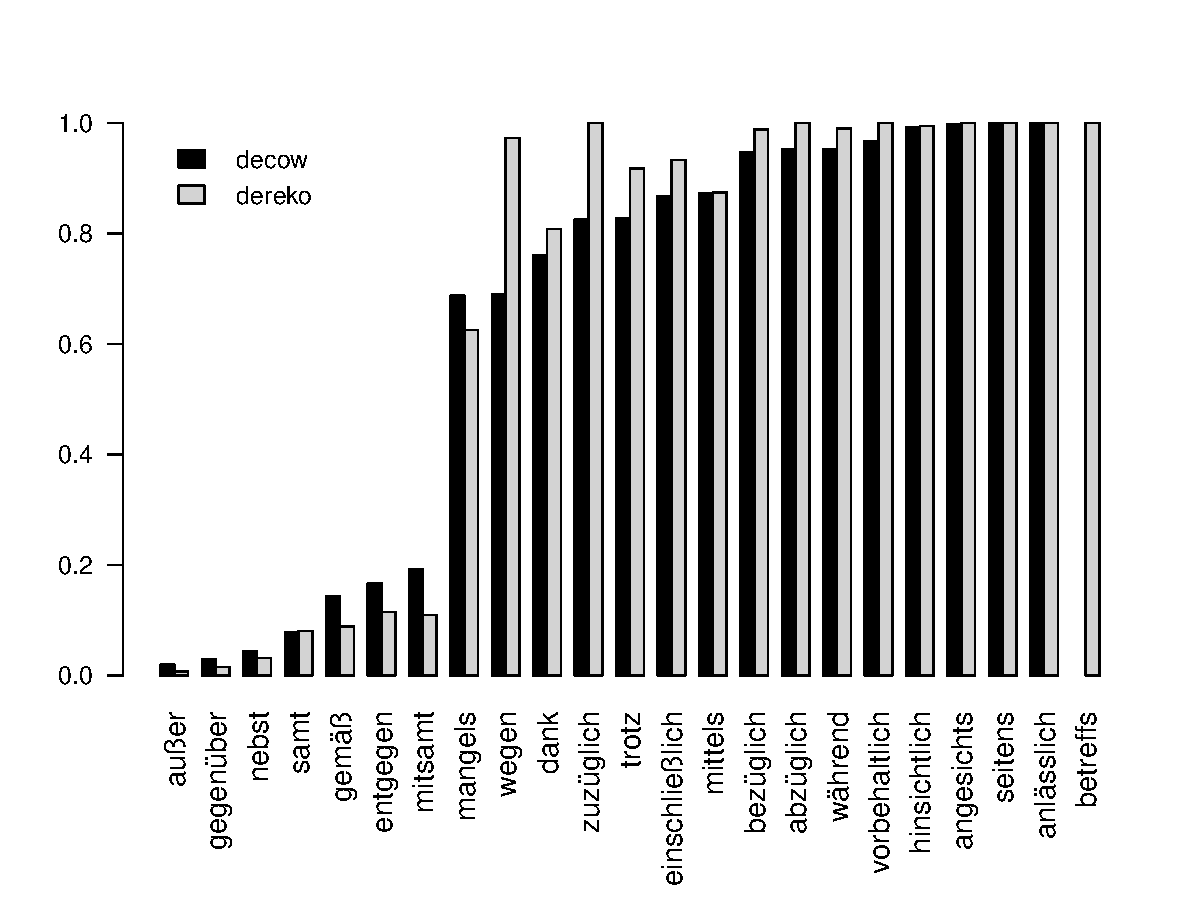
\includegraphics[scale=.7]{../R/plots/prep-genitive-proportions}
%   \label{genprops}
%  \caption{Proportion of genitive complements (as opposed to dative) by preposition and corpus, in a sample of 80,000 prepositional phrases from DeReKo and DECOW16B}  
%\end{figure}

Occurrences of these prepositions were extracted from the DeReKo and DECOW16B corpora, restricted to contexts where case (either dative or genitive) is unambiguously marked on the prepositions's complement.
 More precisely, we considered sequences of the form 
 
 \begin{enumerate}
  \item \textsc{preposition} -- \textsc{adjective} -- \textsc{noun} (singular, masc./neut.)\\
      \begin{small}
      \emph{dank soliden Lebens}\\
      \emph{wegen dringendem Tatverdacht}
      \end{small}
  
  \item \textsc{preposition} -- \textsc{article word}\footnote{For the purpose of this study, article words include the definite  and indefinite article ((\emph{der}, \emph{ein}), demonstratives (\emph{dieser}, \emph{jener}), possessives (e.\,g., \emph{mein}, \emph{unser}) as well as \emph{irgendein}.}\\
      \begin{small}
      \emph{wegen des}\\
      \emph{gegenüber dem}
      \end{small}

\end{enumerate}

 
Many, though not all of the selected prepositions show some degree of variation in case assignment.
For our final dataset, we selected only those prepositions where the proportion of either genitive or dative occurrences was between 0.1 and 0.9 in at least one of the corpora.
In other words, the amount of variation must be such that at least 10\% of all occurrences of that preposition show the minority, non-modal (and arguably, non-standard) case category in at least one of the corpora.
By this criterion, only 10 out of the original 23 prepositions were included in the final dataset (\textit{entgegen}, \textit{gem\"a\ss}, \textit{mitsamt}, which typically select a dative complement, as well as \textit{dank}, \textit{einschlie{\ss}lich}, \textit{mangels}, \textit{mittels}, \textit{trotz}, \textit{wegen} and \textit{zuz\"uglich}, which typically select genitive).
For each of these, we randomly selected a maximum of 4,000 occurrences per corpus, and kept only a single instance per document in case there were more than one. The final data set is summarized in Table~\ref{prep-dataset-summary}. Figure~\ref{nscaseprop} shows the proportion of non-standard case in this dataset, by preposition and corpus.

\begin{table}
\label{prep-dataset-summary}  
  \begin{tabular}{llllll}
  \toprule
Preposition          &  nscase.decow & nscase.dereko & n.decow & n.dereko & n.total\\
  \midrule
dank                 &  0.26         & 0.20    & 3786    & 3776   & 7562\\
einschließlich       &  0.13         & 0.08    & 3767    & 3773   & 7540\\
entgegen             &  0.16         & 0.10    & 3747    & 3726   & 7473\\
gemäß                &  0.15         & 0.10    & 3704    & 3790   & 7494\\
mangels              &  0.34         & 0.24    & 3707    & 2311   & 6018\\
mitsamt              &  0.13         & 0.09    & 3728    & 3687   & 7415\\
mittels              &  0.13         & 0.13    & 3742    & 3716   & 7458\\
trotz                &  0.17         & 0.08    & 3781    & 3732   & 7513\\
wegen                &  0.32         & 0.03    & 3713    & 3612   & 7325\\
zuzüglich            &  0.23         & 0.14    & 3351    &  859   & 4210\\
  \bottomrule
  \end{tabular}
\end{table}

\begin{figure}
   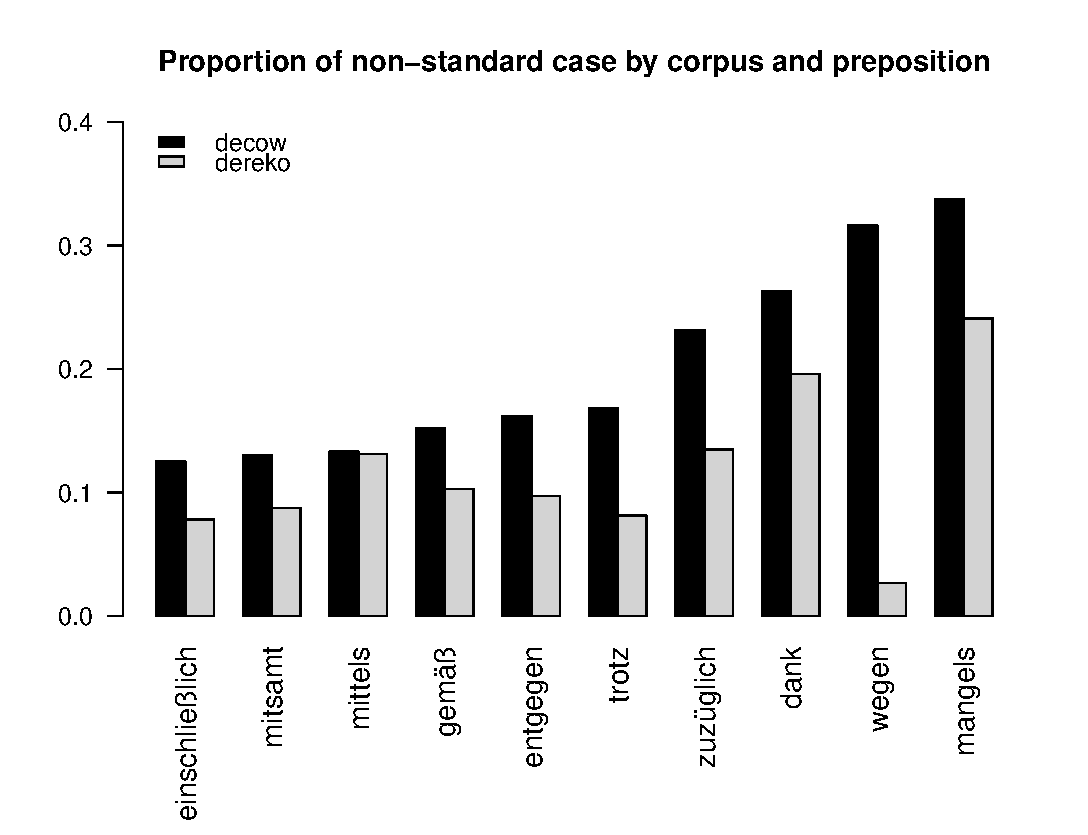
\includegraphics[scale=.7]{../R/plots/nscase-proportions-bw}
   \label{nscaseprop}
  \caption{Proportion of non-standard case by preposition and corpus, in a sample of 73,922 prepositional phrases from DeReKo and DECOW16B}  
\end{figure}

We first specify two logistic regression models that predict the probability of observing the non-modal/non-standard case category, and which do not distinguish between individual prepositions.
First, we use the set of COReX variables, represented as $c_1$ \ldots $c_{60}$ in equation~\ref{glm-allpreps-corex}.

\marginpar{Variable name}
\begin{equation}
\label{glm-allpreps-corex}
  P(nonstandard.case=1) = logit^{-1}(\alpha + \beta_1 c_1 + \beta_2 c_2 + \dots + \beta_{60} c_{60})
\end{equation}


Of the resulting coefficient estimates, 32 are different from 0 at p < 0.05. The Nagelkerke Pseudo-R$^2$ score for this model is 0.28.

For comparison, we use the document factor scores from the factor analysis as shown in equation~\ref{glm-allpreps-fa} (where the terms $f_1$ \ldots $f_7$ represent the factor scores of factors 1 through 7). In this model, all coefficient estimates are significant at the 0.05 level, however, the Nagelkerke R$^2$ score for this model drops to 0.24.

\marginpar{Matrizen oder Laufindex oder Fußnote und erklären}
\begin{equation}
\label{glm-allpreps-fa}
  P(nonstandard.case=1) = logit^{-1}(\alpha + \beta_1 f_1 + \beta_2 f_2 + \dots + \beta_{7} f_{7})
\end{equation}


Next, we consider separate models for each preposition, using first all 60 COReX features as predictors. Figure~\ref{coeffs-corex-individial} illustrates the distribution of estimates for each preposition, for each coefficient with an associated p-value < .05 and absolute value < 5. As is obvious from the plot, coefficient estimates vary greatly, depending on the preposition. 

\begin{figure}
  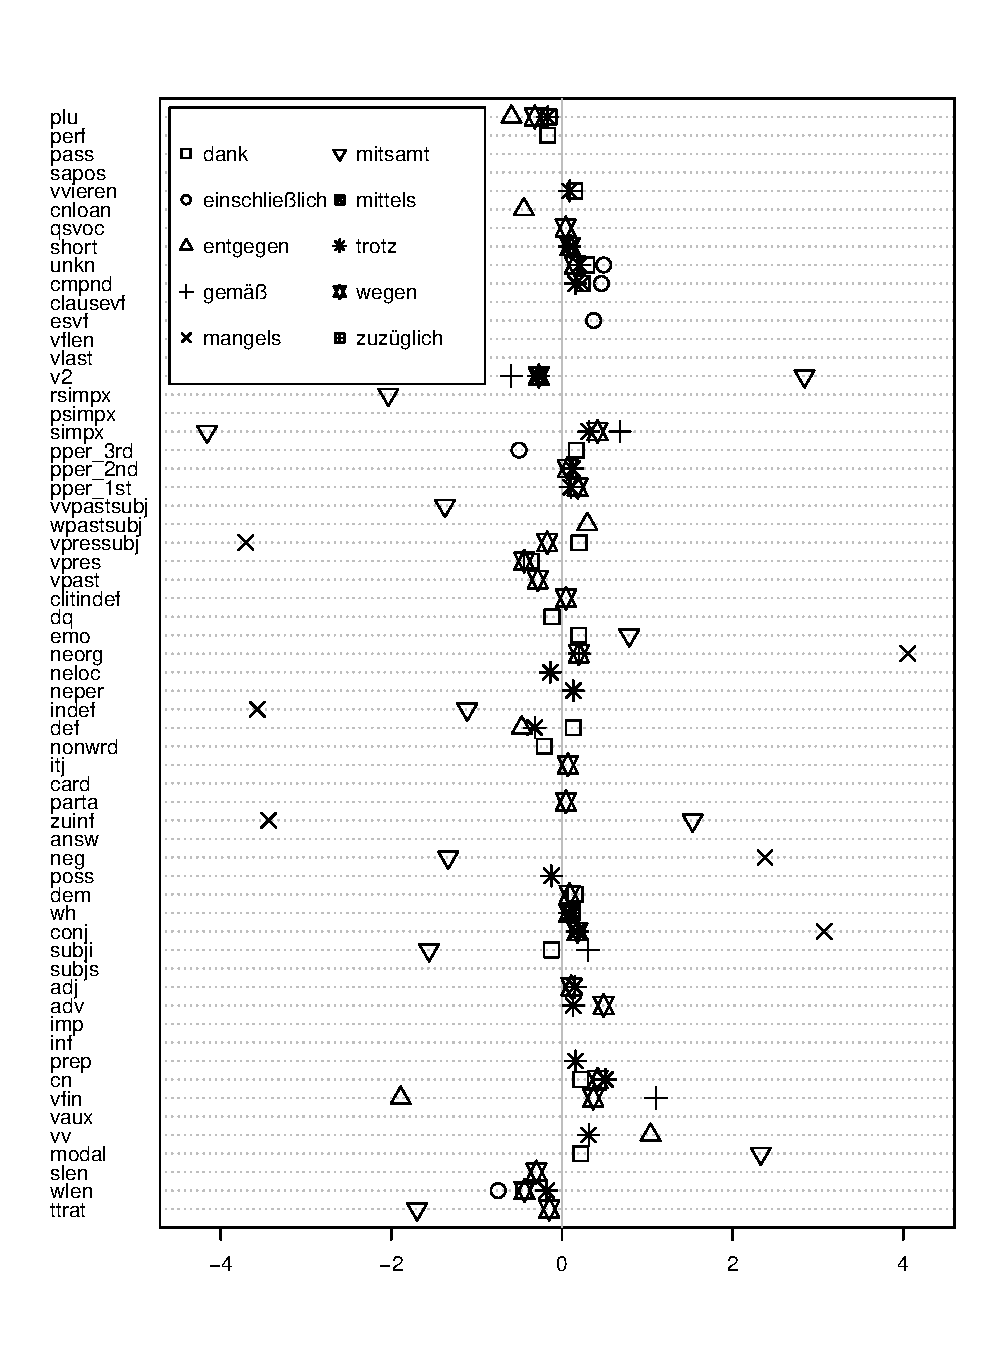
\includegraphics[scale=.9]{../R/plots/prep-individual-coeffs-bw}
  \label{coeffs-corex-individial}
  \caption{COReX features: coefficient estimates with associated p-value $< 0.05$; a separate model was specified for each preposition.}
\end{figure}


\begin{table}
  \begin{tabular}{lrrrrr}
  \toprule
            Preposition  & Total  & nscase & prop.nscase & R2.COReX & R2.FA \\
  \midrule
            dank  & 7562   & 1737   & 0.230    & 0.085   & 0.046  \\
  einschließlich  & 7540   &  767   & 0.102    & 0.112   & 0.061 \\
        entgegen  & 7473   &  969   & 0.130    & 0.067   & 0.028 \\
           gemäß  & 7494   &  953   & 0.127    & 0.028   & 0.003 \\
         mangels  & 6018   & 1808   & 0.300    & 0.214   & 0.135 \\
         mitsamt  & 7415   &  808   & 0.109    & 0.043   & 0.007 \\
         mittels  & 7458   &  985   & 0.132    & 0.088   & 0.037 \\
           trotz  & 7513   &  939   & 0.125    & 0.128   & 0.087 \\
           wegen  & 7325   & 1271   & 0.174    & 0.503   & 0.457 \\
       zuzüglich  & 4210   &  892   & 0.212    & 0.187   & 0.127  \\
  \bottomrule
  \end{tabular}
\end{table}


